\documentclass[conference]{IEEEtran}

% *** CITATION PACKAGES ***
\usepackage[style=ieee]{biblatex} 
\bibliography{refs.bib}

% *** MATH PACKAGES ***
\usepackage{amsmath}
\usepackage{amssymb,amsmath,amsthm, amsfonts}

% *** PDF, URL AND HYPERLINK PACKAGES ***
\usepackage{url}
% correct bad hyphenation here
\usepackage{graphicx}  % needed to include png, eps figures
\usepackage{float}  % used to fix location of images i.e. \begin{figure}[H]
\usepackage{hyperref}

% *** MISCALLENOUS ***
\usepackage{enumitem}
\usepackage{graphicx} % to manage images

% Sections (theorems, propositions, lemmas…) ========================================================================================
\newtheorem{theorem}{Theorem}[section]
\newtheorem{lemma}[theorem]{Lemma}
\newtheorem{corollary}[theorem]{Corollary}
\newtheorem*{conjecture}{\bf Conjecture}
\newtheorem{proposition}[theorem]{Proposition}
% \numberwithin{theorem}{section} % To display the section number in the theorem

\theoremstyle{definition}
\newtheorem{definition}[theorem]{Definition}
\newtheorem{assumption}[theorem]{Assumption}
\newtheorem{exercise}{Exercise}
\newtheorem*{solution}{Solution}
\newtheorem*{answer}{Answer}
\newtheorem*{claim}{Claim}

\theoremstyle{remark}
\newtheorem*{theoremno}{{\bf Theorem}}
\newtheorem*{remark}{Remark}
\newtheorem*{example}{Example}
\newtheorem*{hint}{Hint}



% Commands ========================================================================================
\def\bb#1{\mathbb{#1}}
\def\cal#1{\mathcal{#1}}
\def\frak#1{\mathfrak{#1}}
\def\rm#1{\mathrm{#1}}
\def\bf#1{\mathbf{#1}}
\newcommand{\C}{\mathbb{C}}
\newcommand{\R}{\mathbb{R}}
\newcommand{\N}{\mathbb{N}}
\newcommand{\Z}{\mathbb{Z}}
\newcommand{\Q}{\mathbb{Q}}
\newcommand{\K}{\mathbb{K}}
\newcommand{\bbP}{\mathbb{P}}
\newcommand{\F}{\mathcal{F}}
\newcommand{\calP}{\mathcal{P}}
\newcommand{\G}{\mathcal{G}}
\newcommand{\calL}{\mathcal{L}}
\newcommand{\calC}{\mathcal{C}}
\newcommand{\calN}{\mathcal{N}}
\newcommand{\calF}{\mathcal{F}}
\newcommand{\calE}{\mathcal{E}}
\newcommand{\frakA}{\mathfrak{A}}
\newcommand{\frakS}{\mathfrak{S}}
\newcommand{\esp}{\mathbb{E}}
% \P = caracs spéciaux,\S = paragraphe, \L = L barre

% Already exists : ker, partie Im, Re, min, max, inf, sup, log, exp, sin, sinh, cos, cosh,, tan lim, liminf, limsup
\DeclareMathOperator{\Id}{Id}
\DeclareMathOperator{\Hom}{Hom}
\DeclareMathOperator{\Ima}{Im}
\DeclareMathOperator{\Homeo}{Homeo}
\DeclareMathOperator{\Aut}{Aut}
\DeclareMathOperator{\Bij}{Bij}
\DeclareMathOperator{\Isom}{Isom}
\DeclareMathOperator{\GL}{GL}
\DeclareMathOperator{\End}{End}
\DeclareMathOperator{\rang}{rang}
\DeclareMathOperator{\rank}{rank}
\DeclareMathOperator{\vol}{vol}
\DeclareMathOperator{\sgn}{sgn}
\DeclareMathOperator{\var}{Var}
\DeclareMathOperator{\erf}{erf}
\DeclareMathOperator{\spec}{spec}
\DeclareMathOperator{\diag}{diag}
\DeclareMathOperator{\pgcd}{pgcd}
\DeclareMathOperator{\pgdc}{pgdc}

% Probability stuff
\DeclareMathOperator{\Geom}{Geom}
\DeclareMathOperator{\Bin}{Bin}
\DeclareMathOperator{\Exp}{Exp}
\DeclareMathOperator{\Ber}{Ber}
\DeclareMathOperator{\Student}{Student}
\DeclareMathOperator{\Poi}{Poi}

% Calculus stuff
\newcommand{\czero}{\calC^0}
\newcommand{\cone}{\calC^1}
\newcommand{\ctwo}{\calC^2}
\newcommand{\cinf}{\calC^{\infty}}
\newcommand{\series}[2]{\sum_{#1}^{\infty}#2}
\newcommand{\intt}[4]{\int_{#1}^{#2}#3\mathrm{d}#4}
\newcommand{\ddt}[1]{\frac{\mathrm{d}#1}{\mathrm{dt}}}
\newcommand{\deldt}[1]{\frac{\partial#1}{\partial\mathrm{t}}}
\newcommand{\rmd}[1]{\mathrm{d}#1}
\newcommand{\inv}[1]{#1^{-1}}
\newcommand{\dx}{\rmd x}
\newcommand{\dy}{\rmd y}
\newcommand{\dz}{\rmd z}
\newcommand{\dt}{\rmd t}
\newcommand{\du}{\rmd u}
\newcommand{\dv}{\rmd v}
\newcommand{\ds}{\rmd s}
\newcommand{\dxy}{\rmd xy}
\newcommand{\dyz}{\rmd yz}
\newcommand{\dyx}{\rmd yx}
\newcommand{\dzy}{\rmd zy}
\newcommand{\dzx}{\rmd zx}
\newcommand{\dxz}{\rmd xz}
\newcommand{\gtinf}[1]{\underset{#1\to\infty}{\longrightarrow}}

% algebra stuff
\newcommand{\bigpeter}[1]{\Big\langle#1\Big\rangle}
\newcommand{\peter}[1]{\langle#1\rangle}
\newcommand{\transp}[1]{#1^t}
\newcommand{\sm}[4]{\begin{psmallmatrix}#1&#2\\#3&#4\end{psmallmatrix}}
\newcommand{\map}[4]{
	\begin{matrix}
		#1&\to&#2\\#3&\mapsto&#4
	\end{matrix}
}



\begin{document}

% paper title
\title{Study of the properties of the Relaxed Recentered Log-Barrier function based Nonlinear Model Predictive Control (RRLB NMPC)}

% author names 
\author{Tudor Oancea}% <-this % stops a space
        

% make the title area
\maketitle

% As a general rule, do not put math, special symbols or citations
% in the abstract or keywords.
\begin{abstract}
    Lorem ipsum dolor sit amet.
\end{abstract}

\section{Introduction}
Lorem ipsum dolor sit amet.




\section{Background material}

\subsection{The RRLB MPC}

In this paper we consider the control of general nonlinear $\ctwo$ time-invariant discrete-time dynamical systems of the form 
\begin{equation}
	\label{eq:sys}
	x(k+1) = f(x(k),u(k)),\, x(k)\in\R^{n_x}, u(k)\in\R^{n_u},
\end{equation}
that we are also going to abbreviate $x^+ = f(x,u)$ and that we want to stabilize around a steady state that we can take without loss of generality as the origin. 
This means that $f(0,0) = 0$.
We further suppose that our the states and control inputs are constrained in the form of compact polytopic constraints:
\begin{equation}
	\label{eq:constr}
	\begin{aligned}
		\mathcal{X} &= \{x\in\R^{n_x} \mid C_x x \leq d_x \},\\
		\mathcal{U} &= \{u\in\R^{n_u} \mid C_u u \leq d_u\},
	\end{aligned}
\end{equation}
where $C_x, C_u \in \R^{q_x \times n_x}, \R^{q_u \times n_u}$ are matrices and $d_x, d_u \in \R^{q_x}, \R^{q_u}$ are vectors.
These constraints can be translated into \textit{(weight) recentered log-barrier functions} that are added in the objective function of the MPC to keep the states and control inputs inside the feasible set.

We can however relax these functions as proposed in \cite{RRLB-linear-MPC} and define \textit{relaxed recentered log-barrier functions} (or \textit{RRLB functions}) $B_x$ and $B_u$.
We recall below the definitions only for $B_x$ (since they are similar for $B_u$):
\begin{align}
	B_x(x)&=\sum_{i=1}^{q_x}(1+w_{x,i})B_{x,i}(x),\\
	\text{ with }B_{x,i}(x)&=\begin{cases}
		\log(d_{x,i})-\log(d_{x,i}-\rm{row}_i(C_x)x)\\
		~~~~\text{if }d_{x,i}-\rm{row}_i(C_x)x>\delta\\
		\beta(d_{x,i}-\rm{row}_i(C_x)x;\delta)\\
		~~~~\text{otherwise},
	\end{cases}
\end{align}
Here $\delta$ is called the \textit{relaxation parameter} and $\beta$ is the function that extends the usual log-barrier functions to the whole space in a twice continuously differntiable fashion.
The simplest example for such a function $\beta$ is:
\begin{equation}
	\label{eq:beta}
	\beta(z;\delta)=\frac{1}{2}\left[ \left( \frac{z-2\delta}{\delta} \right)^2-1 \right]-\log(\delta)\,.
\end{equation}

The weights $w_{x,i}, i=1,\dots,q_x$ are chosen such that $B_x(0)=0$ and $\nabla B_x(0)=0$.
These equations only have solutions if $0<\delta\leq\min\left\{d_{x,1},\ldots,d_{x,q_x},d_{u,1},\ldots,d_{u,q_u}\right\}$\,, which is always possible if $0\in\cal{X}$ and $0\in\cal{U}$\,.
An illustration of this relaxation procedure can be found in figure~\ref{fig:RRLB-functions} found in \cite{RRLB-linear-MPC}.

\begin{figure}
	\centering
	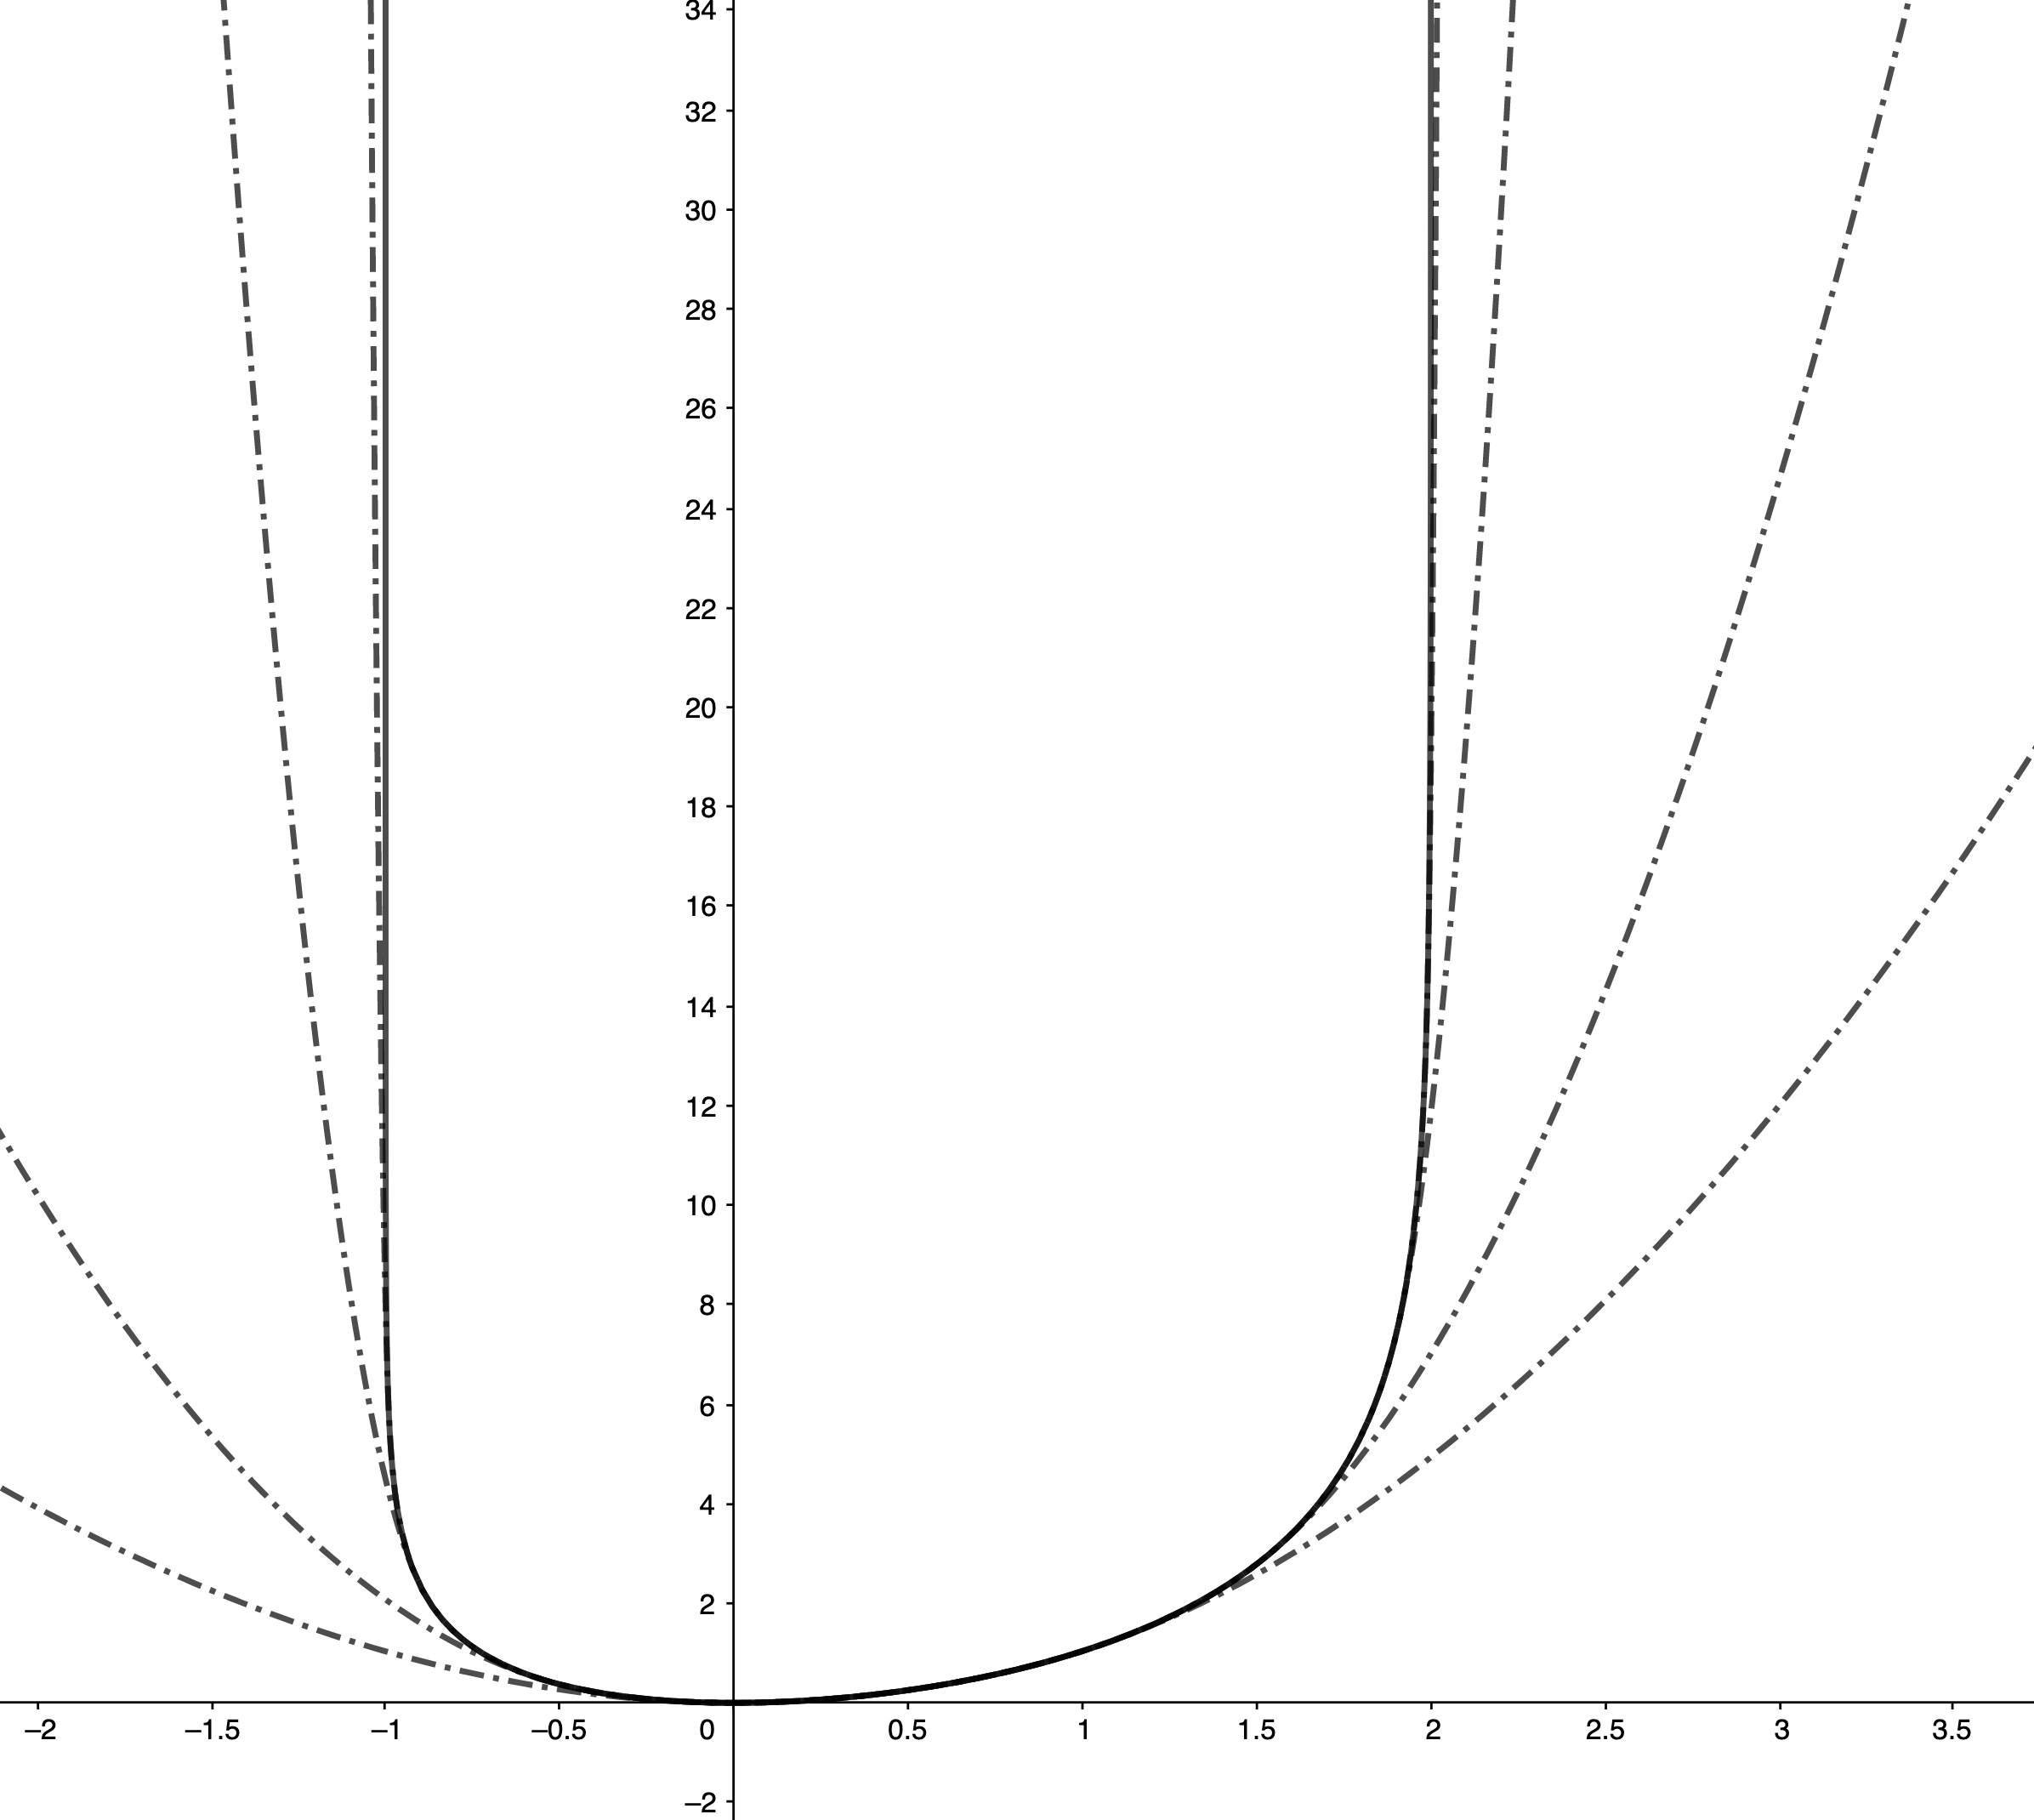
\includegraphics[width=0.5\textwidth]{images/rrlb-functions.png}
	\caption{\textit{(Left)}: Principle of relaxed log barrier function based on quadratic relaxation. (\textit{Right}): Regular weight recentered log barrier function (solid line) and RRLB function for $\delta\in\left\{ 0.01,0.1,0.5,1 \right\}$ for the constraint $z\in\R,~-1\leq z\leq 2$}
	\label{fig:RRLB-functions}
\end{figure}

Now if we consider the following regular nonlinear MPC:
\begin{align}
	\begin{split}
		\label{eq:NMPC}
		V(x)=\underset{\bf{x},\bf{u}}{\min} &\quad J(\bf{x}, \bf{u})=\sum_{k=0}^{N-1}l(x_k,u_k)~+~F(x_N),\\
		\text{s.t.} &\quad x_0=x,\\
		&\quad x_{k+1}=f(x_k,u_k),~k=0,\ldots,N-1,\\
		&\quad x_k\in\cal{X},~k=0,\ldots,N,\\
		&\quad u_k\in\cal{U},~k=0,\ldots,N-1,
	\end{split}
\end{align}
where the stage costs $l(x,u)=x^TQx+u^TRu$ and the terminal cost $F(x)=x^TPx$ are positive definite quadratic functions, we can define the nonlinear \textit{RRLB MPC}:
\begin{align}
	\begin{split}\label{eq:RRLB-NMPC}
		\tilde{V}(x)=\underset{\bf{x},\bf{u}}{\min} &\quad \tilde{J}(\bf{x},\bf{u})=\sum_{k=0}^{N-1}\tilde{l}(x_k,u_k)~+~\tilde{F}(x_N)\\
		\text{s.t.} &\quad x_0=x,\\
		&\quad x_{k+1}=f(x_k,u_k),~k=0,\ldots,N-1,
	\end{split}
\end{align}
where $\epsilon$ is the barrier parameter and the new stage and terminal costs are defined by $\tilde{l}(x,u)=l(x,u)+\epsilon B_x(x)+\epsilon B_u(u)$ and $\tilde{F}(x)=x^T\tilde{P}x$ (for a matrix $\tilde{P}$ that will be determined in such a way that the control law given by the MPC yields an asymptotically stable system).

\subsection{RRLB MPC in the case of linear dynamics}

When we consider the RRLB MPC~\eqref{eq:RRLB-NMPC} in the case of linear dynamics $x^+=f(x,u)=Ax+Bu$, we know the two following theorems to be true:

\begin{theorem}[Theorem 5 in \cite{RRLB-linear-MPC}]
	\label{nominal-stability-linear-case}
	Suppose that the pair $(A,B)$ is stabilizable and that the matrix $P$ is chosen as the unique positive definite solution to the following modified DARE:
	\begin{equation}
		% \label{eq:modified-DARE-linear}
		P=A^TPA-A^TPB(R+\epsilon M_u+B^TPB)^{-1}B^TPA+Q+\epsilon M_x
	\end{equation}
	where $M_x=\nabla^2 B_x(0)$ and $M_u=\nabla^2 B_u(0)$\, are the hessian of the RRLB functions at the origin.

	Then for any initial state $x(0)\in\R^{n_x}$, the control law given by the MPC yields a globally asymptotically stable system.
\end{theorem}

\begin{theorem}[Lemma 5 in \cite{RRLB-linear-MPC}]
	\label{constraint-satisfaction-guarantee-linear-case}
	In the same conditions as in the previous theorem, there is a neighborhood $\cal{X}_N(\delta)$ of the origin such that for any initial state $x(0)\in\cal{X}_N(\delta)$, all the constraint will be satisfied along the closed-loop trajectories.
	Furthermore, the set $\cal{X}_N(\delta)$ is given explicitly by:
	\begin{multline}
		\cal{X}_N(\delta)=\big\{x\in\cal{X}~|~\tilde{V}(x(0))-x(0)^TP_{\rm{LQR}}x(0)\\\leq\min\{\beta_x(\delta),\beta_u(\delta)\}\big\}
	\end{multline}
	where $P_{\rm{LQR}}$ is the solution to the classical DARE and
	\begin{align}
		\beta_x(\delta)&=\underset{i,x}{\min}\left\{ B_x(x)~|~\rm{row}_i(C_xx)=d_{x,i} \right\},\\
		\beta_u(\delta)&=\underset{i,u}{\min}\left\{ B_u(u)~|~\rm{row}_i(C_uu)=d_{u,i} \right\}
	\end{align}
	bruh
\end{theorem}
Additional results were proven in the linear case, such as the existence of a procedure to find $\delta$ such that the maximum constraint violation along the closed-loop trajectories is bounded by a pre-defined tolerance.
In the nonlinear case, however, we will not be able to prove such powerful results because of the lack of knowledge on the error terms that appear in the dynamics.

\section{Theoretical properties of nonlinear RRLB MPC}
\label{sec:RRLB-theoretical-properties}

In this section, for an initial state $x\in\R^{n_x}$ we will denote by $\tilde{\bf{x}}(x)=\left\{ \tilde{x}_0(x)=x,\tilde{x}_1(x),\ldots,\tilde{x}_N(x) \right\}$ and $\tilde{\bf{u}}(x)=\left\{ \tilde{u}_0(x),\tilde{u}_1(x),\ldots,\tilde{u}_{N-1}(x) \right\}$ the optimal sequences of states and controls found by the RRLB MPC.
When no confusion is possible we will drop the "$(x)$".

\subsection{Nominal asymptotic stability}\label{sec:RRLB-nominal-stability}

\begin{lemma}\label{thm:Lipschitzianity}
	Consider the RRLB MPC~\eqref{eq:RRLB-NMPC} that can be written as the unconstrained problem
	$$\tilde{V}(x)=\underset{\bf{u}}{\min} \quad \hat{J}(x,\bf{u})$$
	where $\hat{J}(x,\bf{u})=\tilde{l}(x,u_0)+\tilde{l}(f(x,u_0),u_1)+\cdots+\tilde{F}(f(f(...),u_{N-1}))$\,.
	If for a certain initial state $\bar{x}$ we suppose that $D_\bf{u}\hat{J}(\bar{x},\tilde{\bf{u}}(\bar{x}))=0$ and $\nabla_{\bf{u}\bf{u}}^2\hat{J}(\bar{x}, \tilde{\bf{u}}(\bar{x}))\succ 0$ (the matrix is positive definite) then in a neighborhood of $\bar{x}$ we have:
	\begin{itemize}[label=\textbullet]
		\item $\forall k=0,\ldots,N-1,\quad \|\tilde{u}_k(x)\|=O(\|x\|)$
		\item $\forall k=1,\ldots,N,\quad \|\tilde{x}_k(x)\|=f(f(\ldots,u_{k-2}),u_{k-1})=O(\|x\|)$
	\end{itemize}
\end{lemma}
\begin{proof}
	We can use the proof of the Theorem 4.2 in \cite{lectures-parametric-optimization} to argue that each $\tilde{x}_k$ and $\tilde{u}_k$ is continuously differentiable in a closed neighborhood of the origin.
	Therefore, by continuity their gradient is bounded on this neighborhood and they are Lipschitz.
\end{proof}

\begin{theorem}\label{thm:nominal-stability}
	Let's consider the problem~\eqref{eq:RRLB-NMPC} and assume the following:
	\begin{enumerate}
		\item If we denote the objective function as $J(x,\bf{u})$ as in Lemma~\ref{thm:Lipschitzianity}, we have $D_\bf{u}J(0,\bf{u}(0))=D_\bf{u}J(0,0)=0$ and $\nabla^2_{\bf{u}\bf{u}}J(0,\bf{u}(0))=\nabla^2_{\bf{u}\bf{u}}J(0,0)\succ 0$

		\item When linearizing the system dynamics around the origin and letting $A=D_xf(0,0),$ $B=D_uf(0,0)$, we suppose that the pair $(A,B)$ is stabilizable.
		This implies in particular that there exists a stabilizing cost $K$, i.e. a matrix such that $A_K:=A+BK$ only has eigenvalues in the unit disk.

		\item The matrix $\tilde{P}$ defining the terminal costs is the unique positive definite solution to the following Lyapunov equation:
		\begin{equation}
			\label{eq:Lyapunov}
			\tilde{P}=A_K^T\tilde{P}A_K+\mu \tilde{Q}_K
		\end{equation}
		where $\mu>1$ and $\tilde{Q}_K=\underbrace{Q+\epsilon M_x}_{=:\tilde{Q}}+K^T(\underbrace{R+\epsilon M_u}_{=:\tilde{R}})K$\,.
	\end{enumerate}
	Then the dynamical system $x^+=f(x,\tilde{u}_0(x))$ is locally asymptotically stable, i.e. for all initial state in a neighborhood of the origin, the control law given by the RRLB MPC yields an asymptotically stable system.
\end{theorem}

\begin{remark}~
	To identify the matrix $K$, we can approximate $\mu\approx 1$ and solve the following classical DARE:
	\begin{equation}
		\label{eq:modified-DARE}
		\begin{cases}
			K=-(\tilde{R}+B^T\tilde{P} B)^{-1}B^T\tilde{P} A,&\\
			\tilde{P}=A_K^T\tilde{P} A_K+\tilde{Q}_K\,.
		\end{cases}
	\end{equation}
	The factor $\mu$ is very important in theory but in practice could be taken very close to 1 or actually equal to 1.
\end{remark}

\begin{proof}~
	To prove local asymptotic stability we will show that $\tilde{V}$ is a Lyapunov function in a neighborhood of the origin.
	First, using the recentering of the RRLB functions, we can write the Taylor expansion of the stage costs $\tilde{l}$:
	\begin{align*}
		\tilde{l}(x,u)&=x^T[\nabla_{xx}^2\tilde{l}(0,0)] x+u^T[\nabla_{uu}^2\tilde{l}(0,0)]u+O(\|x\|^3+\|u\|^3)\\
		&=x^T\tilde{Q}x+u^T\tilde{R}u+O(\|x\|^3+\|u\|^3)\\
		&\implies\tilde{l}(x,Kx)=x^T\tilde{Q}_Kx+O(\|x\|^3)\,.
	\end{align*}
	By the second assumption, we also have $\forall x\in\R^{n_x}$:
	\begin{equation}
		\tilde{F}(A_Kx)+\mu x^T Q_K x-\tilde{F}(x)=0,
	\end{equation}
	and by the same reasoning as in the paragraph 2.5.5 of \cite{MPC-book}, there exists a neighborhood of the origin in which:
	\begin{align}
		&\tilde{F}(f(x,Kx))+x^T Q_K x-\tilde{F}(x)\leq 0\\
		\Longrightarrow&\tilde{F}(f(x,Kx))-\tilde{F}(x)+\tilde{l}(x,Kx)=O(\|x\|^3)\,.
	\end{align}
	What's more, by lemma \ref{thm:Lipschitzianity}, the predicted states are all Lipschitz with respect to the initial state, so we can choose an even smaller neighborhood such that $\tilde{x}_N(x)$ is also in it.

	Now using the optimal sequence of states and controls of the RRLB MPC starting at $x$, we can construct new feasible sequences for the problem starting at $\tilde{x}_1(x)$ as
	$\bf{x}'=(\tilde{x}_1,\ldots,\tilde{x}_N,f(\tilde{x}_N,K\tilde{x}_N))$ and $\bf{u}'=(\tilde{u}_1,\ldots,\tilde{u}_{N-1},K\tilde{x}_N)$\,.
	Then we obtain:
	\begin{align*}
		\tilde{V}(\tilde{x}_1)&\leq\tilde{J}(\bf{x}',\bf{u}')=\tilde{J}(\tilde{\bf{x}},\tilde{\bf{u}})-\tilde{l}(x,\tilde{u}_0)\\
		&\quad+\tilde{F}(f(\tilde{x}_N,K\tilde{x}_N))-\tilde{F}(\tilde{x}_N)+\tilde{l}(\tilde{x}_N,K\tilde{x}_N)\\
		&=\tilde{V}(x)-O(\|x\|)^2+O(\|x\|^3),
	\end{align*}
	which proves the descent property for $\tilde{V}$\,.
	Finally, it is easy to show that $\tilde{V}$ is lower and upper bounded by coercive quadratic functions (since $Q,R$ are positive definite and $B_x,B_u$ are positive definite and upper bounded by quadratics), so that $\tilde{V}$ is indeed a Lyapunov function in a small neighborhood around the origin.
\end{proof}

\subsection{Constraints satisfaction guarantees}
\label{sec:constraints-satisfaction-guarantees}
\begin{lemma}
	\label{thm:RRLB-bounds-guarantees}
	Consider the RRLB MPC~\eqref{eq:RRLB-NMPC} and an initial state $x(0)$ in the neighborhood given by Theorem~\ref{thm:nominal-stability}.
	Let's denote by $\left\{x(0),x(1),\ldots\right\}$ and $\left\{u(0), u(1),\ldots\right\}$ the closed-loop state and control trajectories (given by $u(k)=\tilde{u}_0(x(k)),~x(k+1)=f(x(k),u(k))$), and define 
	\begin{equation*}	
		\alpha(x(0)):=\frac{1}{\epsilon}\left(\tilde{V}(x(0))-x(0)^TP_{\rm{LQR}}x(0)-\sum_{k=0}^\infty\eta(x(k))\right)
	\end{equation*}
	with $P_{\rm{LQR}}$ is the solution to the classical DARE
	% \begin{multline*}
	% 	P_{\rm{LQR}} = A^T P_{\rm{LQR}} A \\
	% 	- A^T P_{\rm{LQR}} B (R + B^T P_{\rm{LQR}} B)^{-1} B^T P_{\rm{LQR}} A\\
	% 	+ Q + K^T R K
	% \end{multline*}
	, and $\eta(x)=\tilde{l}(\tilde{x}_N(x),K\tilde{x}_N(x))+\tilde{F}(\tilde{x}_N(x))-\tilde{F}(f(\tilde{x}_N(x), K\tilde{x}_N(x)))$.
	Then $\forall k\geq 0$:
	\begin{equation*}
		B_x(x(k)),B_u(u(k))\leq\alpha(x(0))
	\end{equation*}
\end{lemma}

\begin{proof}
	In the proof of theorem~\ref{thm:nominal-stability} we showed that $\forall k\geq 0$:
	\begin{multline*}
		\tilde{V}(x(k+1))-\tilde{V}(x(k))\leq\\
		-\tilde{l}(x(k),u(k))+\tilde{l}(\tilde{x}_N(x(k)), K\tilde{x}_N(x(k)))\\
		-\tilde{F}(\tilde{x}_N(x(k)))+\tilde{F}(f(\tilde{x}_N(x(k)),\tilde{x}_N(x(k)))),
	\end{multline*}
	so by summing for $k=0,1,\dots$, we get a telescopic sum that we can compute using the fact that the system is asymptotically stable so $\lim_{k\to\infty}\tilde{V}(x(k))=0$:
	\begin{align*}
		\tilde{V}(x(0))&\geq\sum_{k=0}^\infty\tilde{l}(x(k),u(k))-\tilde{l}(\tilde{x}_N(x(k)), K\tilde{x}_N(x(k)))\\
		&\qquad+\tilde{F}(\tilde{x}_N(x(k)))-\tilde{F}(f(\tilde{x}_N(x(k)),\tilde{x}_N(x(k))))\\
		&=\sum_{k=0}^\infty l(x(k), u(k))+\epsilon B_x(x(k))+\epsilon B_u(u(k))+\eta(x(k))\\
		&\geq x(0)^TP_{\rm{LQR}}x(0)+\sum_{k=0}^\infty\eta(x(k))\\
		&\qquad+\epsilon\sum_{k=0}^\infty B_x(x(k))+\epsilon\sum_{k=0}^\infty B_u(u(k))\\
	\end{align*}
	Even if we don't know a closed form for $\eta(x(k))$, we know that $\sum_{k=0}^\infty\eta(x(k))$ must be finite because it is bounded by $\tilde{V}(x(0))$\,.
	Now since the RRLB functions are all positive definite, we can easily conclude.
\end{proof}


\begin{lemma}[Lemma 1 in \cite{RRLB-linear-MPC}]
	\label{thm:constraint-set-def-with-RRLB}
	If we define the bounds 
	\begin{align*}
		\beta_x&=\underset{i,x}{\min}\{B_x(x)~|~\rm{row}_i(C_x)x=d_{x,i}\},\\
		\beta_u&=\underset{i,u}{\min}\{B_u(u)~|~\rm{row}_i(C_u)u=d_{u,i}\},
	\end{align*}
	% Even if not written explicitly, the bounds $\beta_x,\beta_u$ depend on the relaxation parameter $\delta$\,.
	then then for all relaxation parameters $\delta$:
	\begin{equation}
		\left\{x~|~B_x(x)\leq\beta_x\right\}\subseteq\cal{X},\quad\left\{u~|~B_u(u)\leq\beta_u\right\}\subseteq\cal{U}
	\end{equation}
\end{lemma}

\begin{theorem}
	In the same setting as lemma~\ref{thm:RRLB-bounds-guarantees}, for any initial state $x(0)$ in the set
	$$\cal{X}_N(\delta):=\left\{x\in\R^{n_x}~|~\alpha(x(0))\leq\epsilon\min\left\{\beta_x,\beta_u\right\}\right\}$$
	there is no state or control constraint violation along the closed loop trajectories.
\end{theorem}

\begin{proof}
	Lemma~\ref{thm:RRLB-bounds-guarantees} implies that for any $x(0)\in\cal{X}_N(\delta)$ and for all $k\geq 0,~\epsilon B_x(x(k))\leq\alpha(x(0))\leq\epsilon\beta_x$ so $B_x(x(k))\leq \beta_x$ and $x(k)\in\cal{X}$.
	The same reasoning applies on the controls.
\end{proof}

\subsection{Variable barrier parameter}
All the previous section assumed that the barrier parameter $\epsilon$ was fixed and did not change throughout the experiment.
However, we could want to gradually decrease it as we converge to actually reach the nominal trajectory.
When we do so, the asymptotic stability is actually preserved.

\begin{lemma}[Monotonicity of the Lyapunov functions when $\epsilon$ decreases]
	Let $\tilde{V}_{\epsilon}$ be the Lyapunov function defined for the RRLB MPC \eqref{eq:RRLB-NMPC} with barrier parameter $\epsilon$.
	Then for any $0<\epsilon_1<\epsilon_2$ we have $\tilde{V}_{\epsilon_1}\leq\tilde{V}_{\epsilon_2}$.
\end{lemma}

\begin{proof}
	If we define by $\tilde{J}_{\epsilon}$ the objective function in \eqref{eq:RRLB-NMPC}, then we have $\forall \bf{x},\bf{u}$:
	\begin{align*}
		&\epsilon_1B_x(x_k)\leq \epsilon_2B_x(x_k),\epsilon_1B_u(u_k)\leq \epsilon_2B_u(u_k)\\
		\implies&\tilde{J}_{\epsilon_1}(\bf{x},\bf{u})<\tilde{J}_{\epsilon_2}(\bf{x},\bf{u})\\
		\implies&\tilde{V}_{\epsilon_1}(x)=\min_{\bf{x},\bf{u}}\tilde{J}_{\epsilon_1}(\bf{x},\bf{u})\leq\min_{\bf{x},\bf{u}}\tilde{J}_{\epsilon_2}(\bf{x},\bf{u}) = \tilde{V}_{\epsilon_2}(x)\\
	\end{align*}
\end{proof}

\begin{theorem}
	Let us suppose that we have run RRLB MPC in closed loop with a decreasing sequence of $\{\epsilon_k\}_{k=0}^\infty$ and that at each step, the associated Lyapunov function is $\tilde{V}_{k}$.
	Then the system is still locally asymptotically stable.
\end{theorem}


\appendix
Lorem ipsum dolor sit amet.

\printbibliography

% that's all folks
\end{document}
